% Chapter 4

\chapter{Prototypation} % Main chapter title

\label{Chapter4} % For referencing the chapter elsewhere, use \ref{Chapter4} 

%----------------------------------------------------------------------------------------

\section{Early version}

This version is very simple and it contains only the basic functionalities. 
The goal of this version are: to understand if this kind of system can be useful for the users, and experiment some technical solutions to create the features needed to achieve the goals. At this stage the application is evidently incomplete, there are numerous deficiencies and inconsistencies and the goals of the Human Machine Interaction are ignored. All this point are corrected in the second version, and this first version can be used to show a "before-after comparison".
GAn Web is a web application (as the name suggests) so the interface is created using HTML and CSS. This languages are very advanced and allows the programmer to create and modify an interface very easily. The framework Bootstrap, used in this project, even improves the performances of these languages. So all the prototypes are directly created by code, without paper-based mock ups.

Following are visible some part of the early prototype, with very simple features.

\begin{enumerate}
\item The homepage:

\begin{figure}[H]
\centering
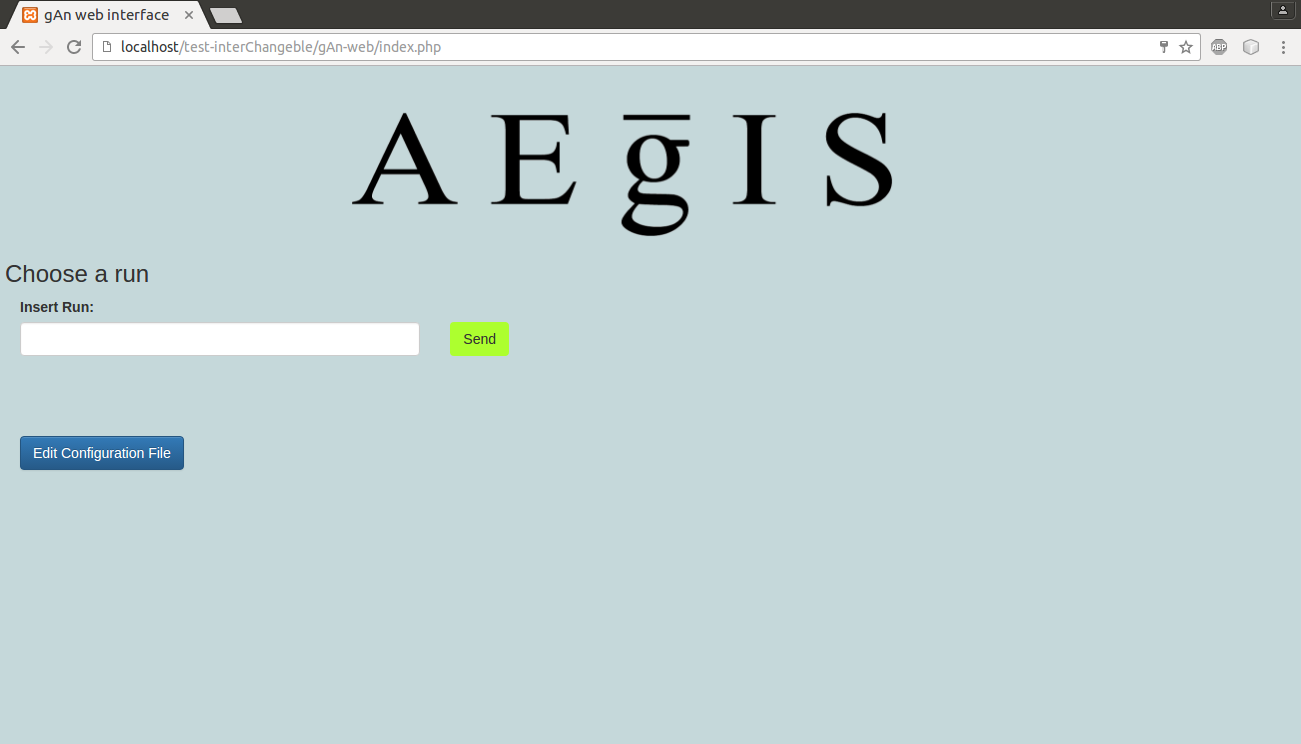
\includegraphics[scale=0.25]{HomePageOLD.png} 
\caption{The early homepage of gAn Web}
\end{figure}

It is quite clear: There is the AEgIS Logo, an input field where the user can insert a run number (only one in this version) and a "Send" button to start the analysis (using gAn). A button "Edit Configuration File" allows the user to  enter in the page dedicated to the configuration of the program.

\item The text output page:

\begin{figure}[H]
\centering
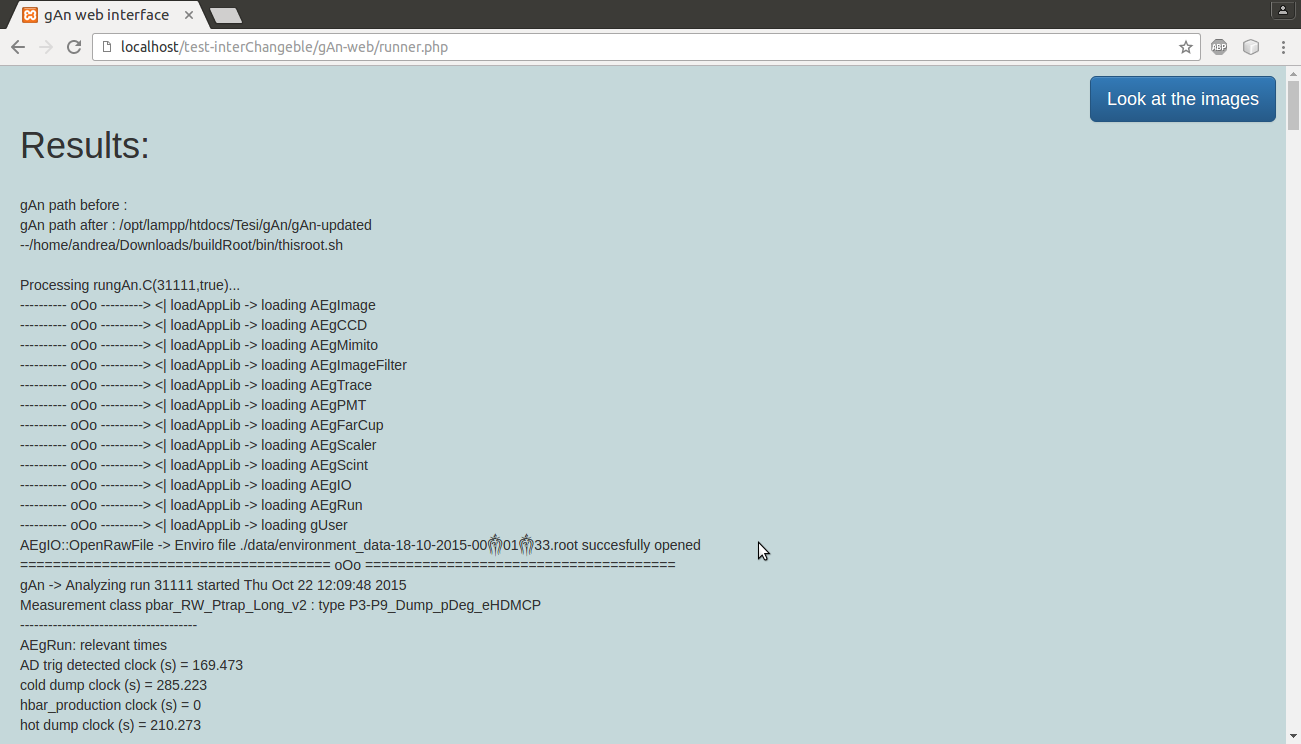
\includegraphics[scale=0.25]{TextOutputOLD.png} 
\caption{The early page related to the textual output of gAn Web}
\end{figure}
  
The textual result of the computation is visible: it seems to be too long and incomprehensible, but for physicists it is quite clear. The graphics is very minimalist, there is only one button: "Look at the images", that sends the user to the page related to the images. 



\item The page related to the images:

\begin{figure}[H]
\centering
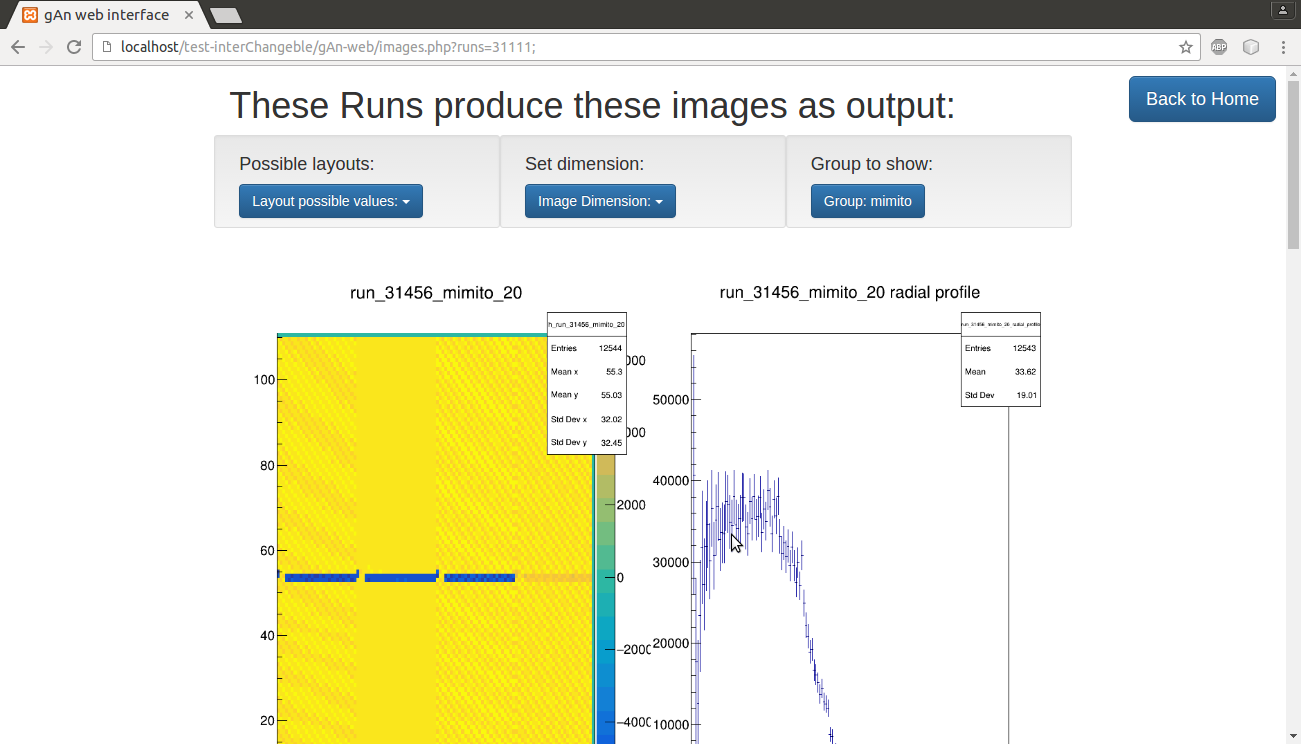
\includegraphics[scale=0.25]{AllImagesPageOLD.png} %TODO %TODO %TODO %TODO %TODO %TODO %TODO %TODO %TODO %TODO %TODO %TODO %TODO %TODO %TODO %TODO %TODO %TODO %TODO %TODO %TODO %TODO %TODO %TODO %TODO %TODO %TODO %TODO %TODO %TODO %TODO %TODO %TODO %TODO %TODO %TODO %TODO %TODO %TODO %TODO %TODO %TODO %TODO %TODO %TODO %TODO %TODO %TODO %TODO %TODO %TODO %TODO %TODO %TODO SISTEMA STOCAZZO DI IMMAGINE
\caption{The page able to show the output images in the early prototype}
\end{figure}   

This page shows the images in a dynamic framework, that the user can edit.
The user the chose by dropdown menus the dimension, the layout ("vertical", if he prefers the images disposed vertically one above the other, "carousel" if he prefers the images organized horizontally, navigable by a "next" button and a "previous" button), the group to show (each image belongs to a group, each group usually is composed by 2-3 images). Clicking on a image the user can open it in a full page version (but it is still a static image, a png).



\item The page that aims to edit the configuration file:

\begin{figure}[H]
\centering
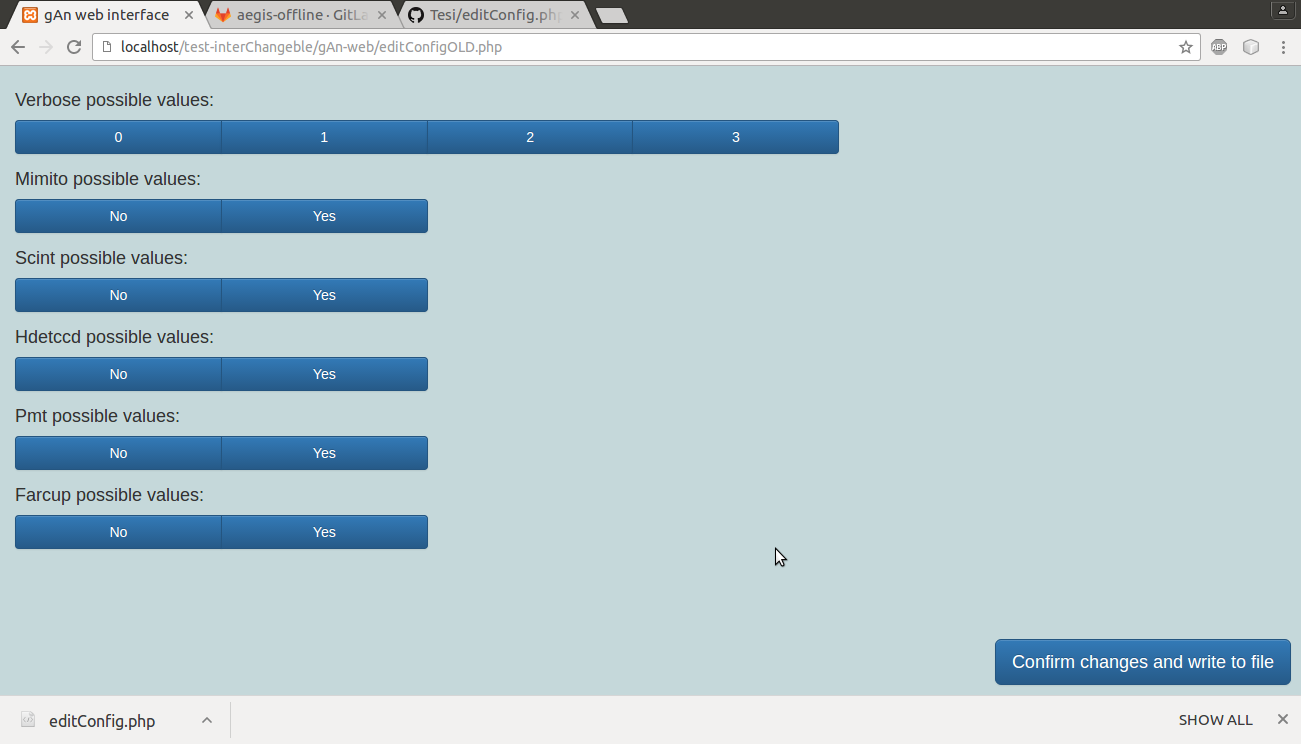
\includegraphics[scale=0.25]{EditConfigOLD.png}  
\caption{The configuration page}
\end{figure}   

This page allows the user to chose by radio buttons (modified using Bootstrap graphic) the value to insert in the configuration file of gAn. Radio buttons force users to insert correct values.    

\end{enumerate}

\section{How the early version can be improved}
The early version's goal is just to be a demo. In particular, it is based on the assumption that the user knows in every moment all about gAn (how does it works,  what is the meaning of each field of the configuration file, etcetera). It can be improved literally in every point, according with the principles of the Human Machine Interaction.


\section{Late version}

The late version is based on the early version, some pages (and functionalities) are added, some existing pages are improved. Following all modifications are explained.

\subsection{Modified pages}
The homepage:

\begin{figure}[H]
\centering
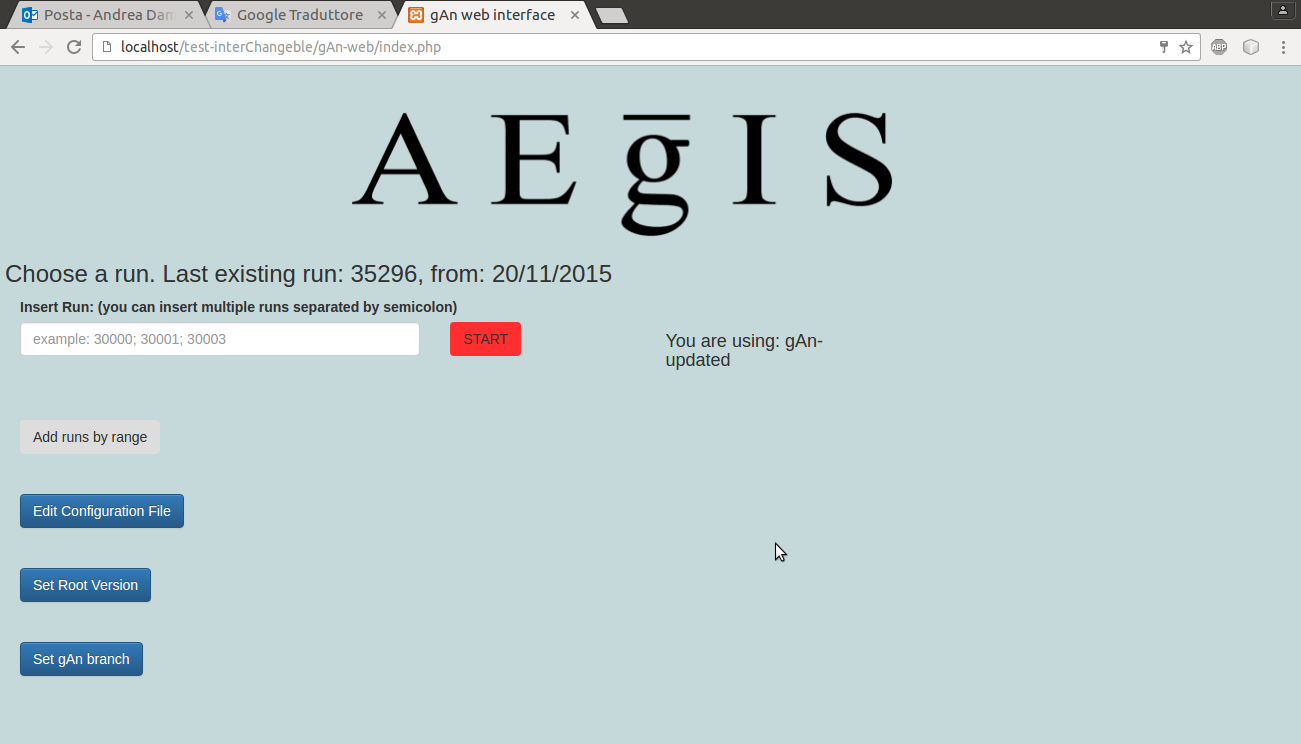
\includegraphics[scale=0.25]{HomePageEmpty.png} 
\caption{The homepage of gAn Web without input}
\end{figure}


\begin{figure}[H]
\centering
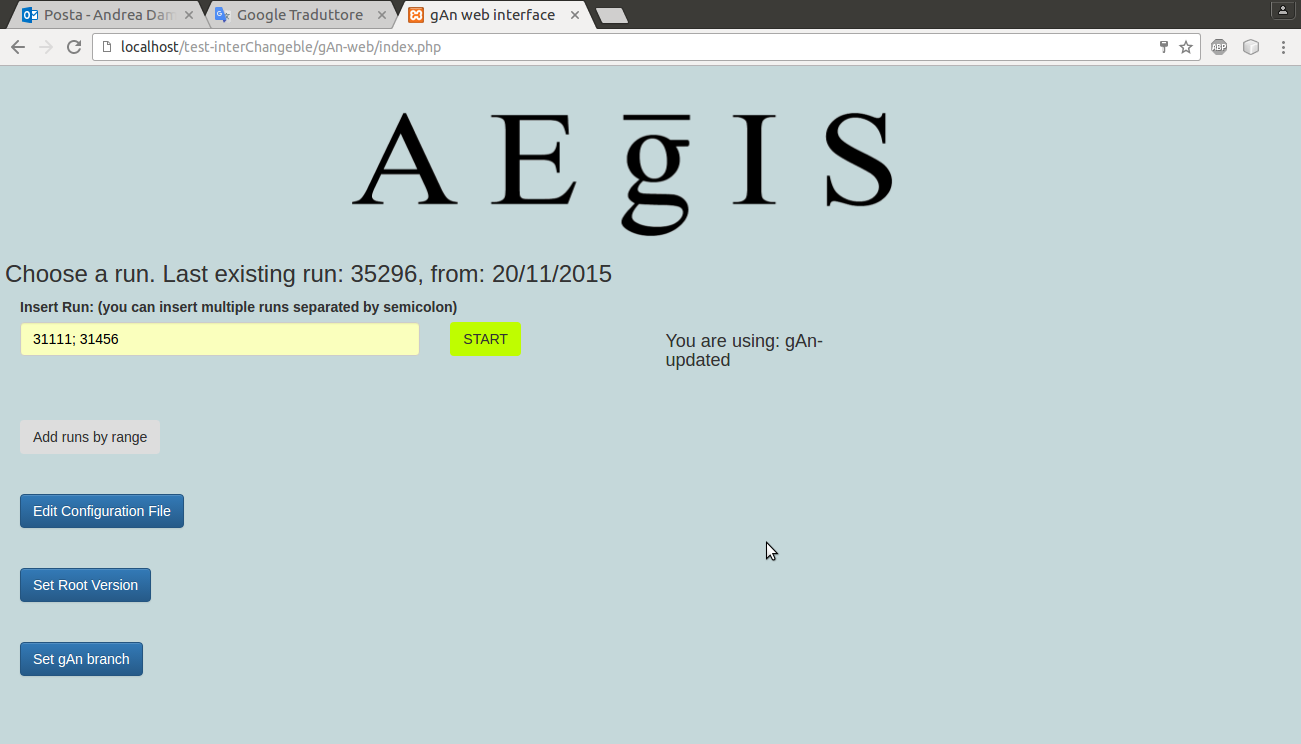
\includegraphics[scale=0.25]{HomePage.png} 
\caption{The homepage of gAn Web ready to start}
\end{figure}

There are some modifications:

\begin{enumerate}

\item The user is informed about what is the last existing run: he can read "last existing run: nnnnn, from dd/mm/yy". This point is important because in most cases the user searches results regarding the lasts 10 runs.

\item The button named "send" was unclear, the word "START" is more clear, the user can immediately understand that the goal of this button is to start gAn. The button is red and unclickable if there are problems (like in the following image) with the inserted runs (or if the input field is empty), green and clickable if there are no problems.	

\begin{figure}[H]
\centering

\includegraphics[scale=0.25]{ErrorInputHomepage.png}  
\caption{The "Start" button is red if the values in the input field are invalid}
\end{figure}

When the user clicks start a progress bar appears. Unfortunately it is very hard to understand exactly how long the computation will last, because different runs can take different time (it depends on the amount of data that the sensors take about the run, and on the workload of the server machine, that is in common with other applications). On average is observed that the computation take five seconds multiplied by the number of selected runs, but if another user asked for that computation before the system already has the results in memory and the computation is faster. A wait of several seconds can be not comfortable for the user, the progress bar is imprecise but ensure to the user that the system is working correctly to ensure the correct answer. In the following image the progress bar:

\begin{figure}[H]
\centering

\includegraphics[scale=0.25]{ProgressBar.png}  
\caption{The progress aimed to make more comfortable the user's waiting}
\end{figure}



\item The input field has a place-holder, that shows to the user how to correctly insert the runs separated by semicolon (there is an automatic system that corrects the inserted values if the separator is not a semicolon)
 
\item It is possible to insert a group of runs selecting them by range (inserting the first and the last): the button "Add runs by range" opens a modal (shown in the image). The user can chose the minimum and the maximum of the range, the system validates the inserted values (maximum must be more that minimum, they must be numbers etcetera).

\begin{figure}[H]
\centering
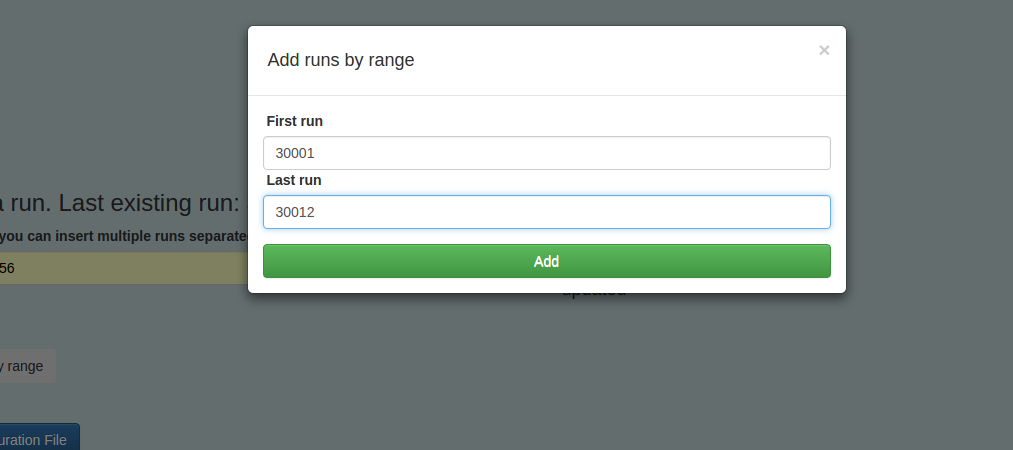
\includegraphics[scale=0.25]{RangeRunsModal.png}  
\caption{The modal opened by clicking the button "Add runs by range"}
\end{figure}

\item There is a little message "You are using: nameOfGAnBranch" that informs the user about which is the branch of gAn used by default if he doesn't change the configuration (the default branch is the last used, because usually when a group of users starts to use a branch, it continues to use it for some days)

\item There are two new buttons: "Chose Root version", "Chose gAn version". These buttons redirect the user to pages able to modify the version of Root and gAn used in the computation.
 
\item Each button and each field have a tooltip: a little explaining text that appears when the user moves the mouse over the object. In this way an inexperienced user can easily understand what each component does.  

\end{enumerate}


The page related to the modifications of the configuration file of gAn:

\begin{figure}[H]
\centering
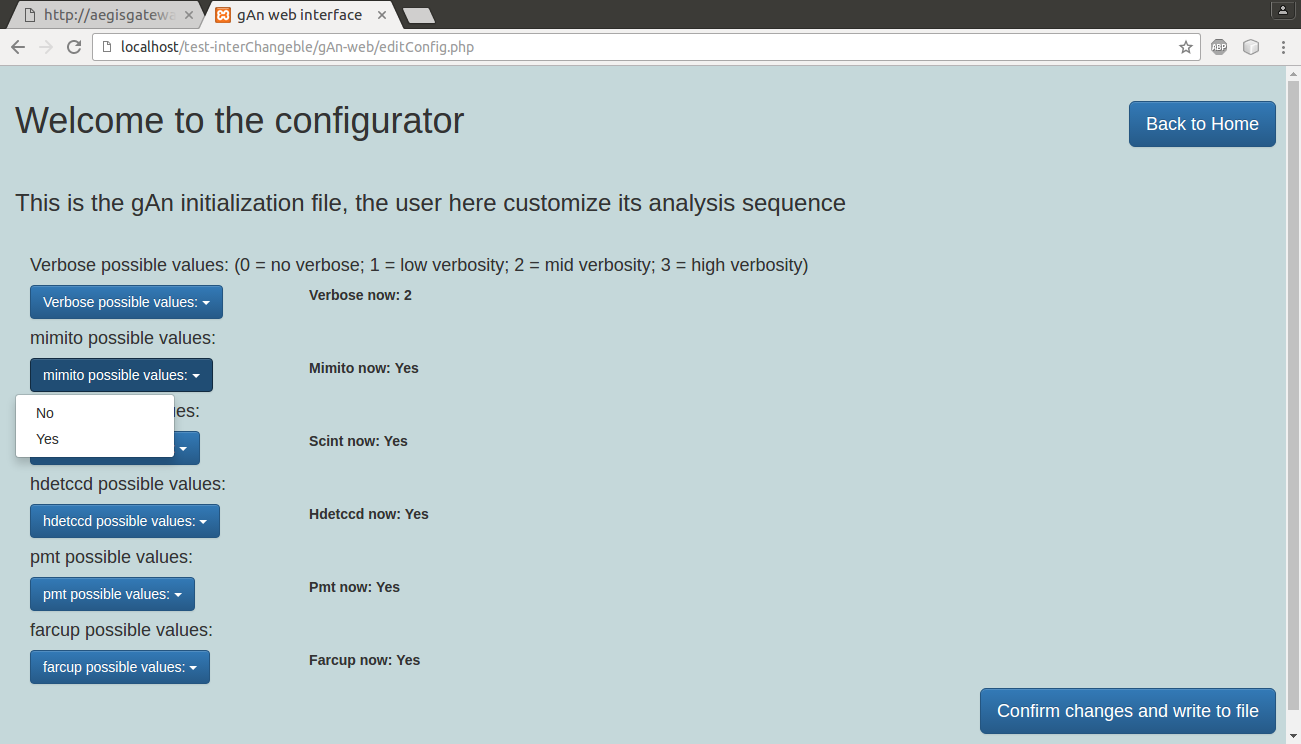
\includegraphics[scale=0.25]{EditConfig.png} 
\caption{The edit-configurator page of gAn Web}
\end{figure}

This page doesn't use anymore radio buttons, because some users ask the developers to use dropdown menus (for aesthetic reasons). The user can read near the button the currently selected value for each field. There aren't tool-tips able to describe the signification of each field here, because the users to which gAn Web is intended have a perfect understanding of the names and the features of each sensor (mimito, scint, farcup, etcetera are sensors).  



The page that shows the textual output of gAn is exposed in the following images, has some modifications:

\begin{figure}[H]
\centering
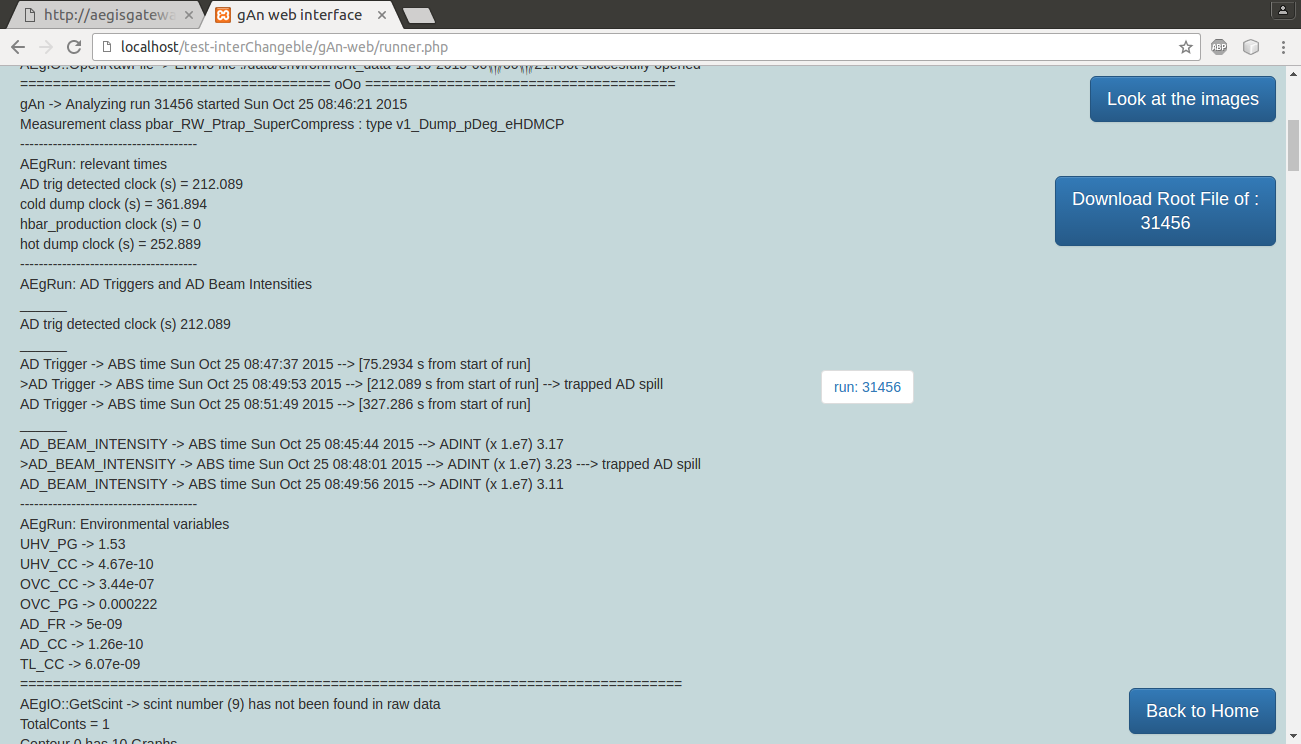
\includegraphics[scale=0.25]{TextOutputPage.png} 
\caption{The page who shows the textual output of gAn}
\end{figure}


\begin{enumerate}
\item The user can chose what results he wants to show on the screen by clicking the corresponding run number from the "navbar", like in the image:

\begin{figure}[H]
\centering
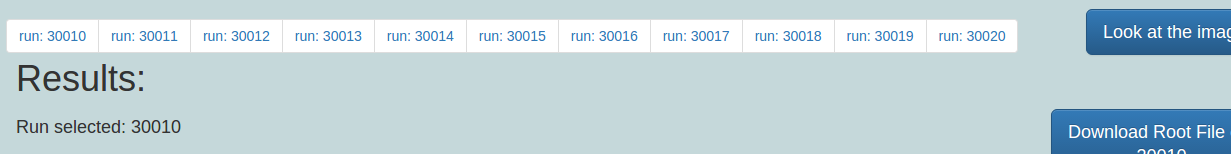
\includegraphics[scale=0.25]{WhichRunNavbar.png} 
\caption{By this "navbar" the user can chose the run results to show}
\end{figure}

This navbar is in fixed position related to the screen, and can be dragged by the user to allow him to decide where put it.

\item "Download Root File of: nnnn" is a button that allows to user to download the semi-processed file .root with some output information regarding the computation.

\item "Back to Home" gives the user the opportunity to directly return to the homepage. 

\item "Back to Home" and "Look at the images" are in a fixed position on the screen: also if the user scrolls down or up the screen he is always able to see these buttons.    

\end{enumerate}
The page that shows in an organized way the images that gAn produces in output. The following image shows the new appearance of the page:



\begin{figure}[H]
\centering
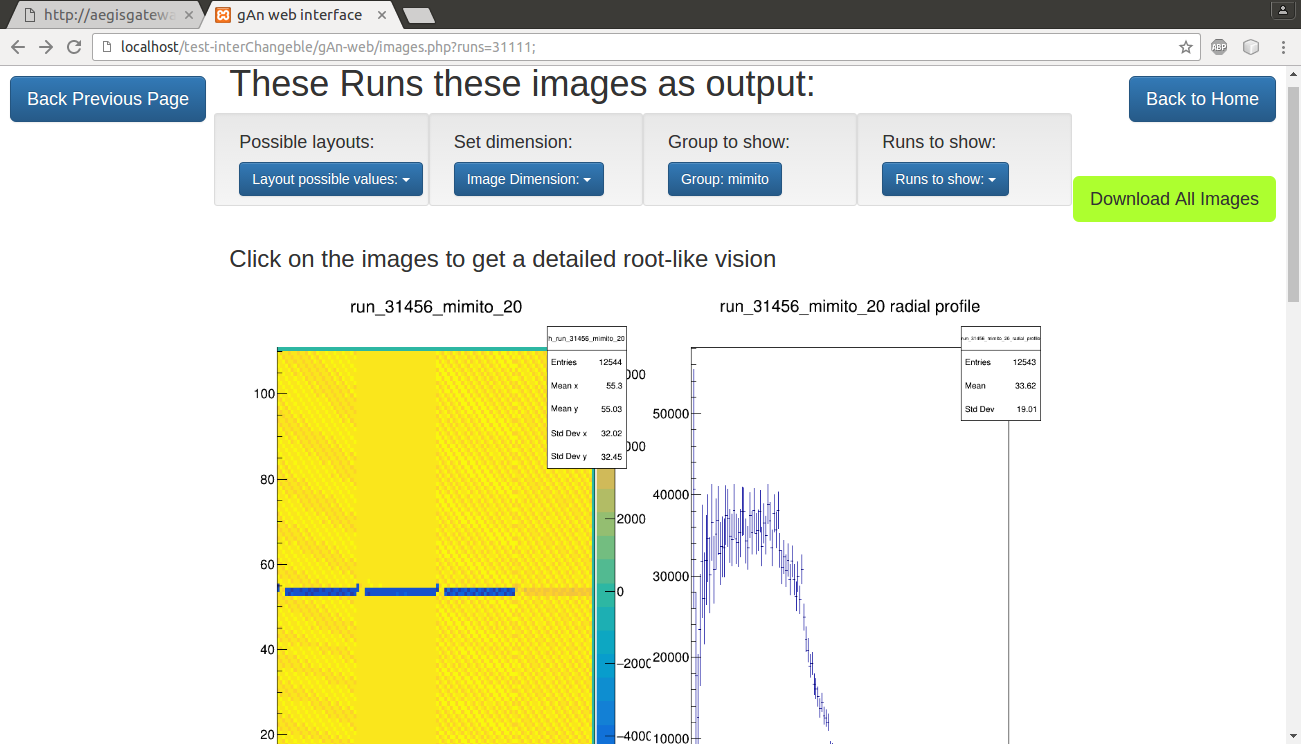
\includegraphics[scale=0.25]{AllImagesPage.png} 
\caption{This page shows all the images that gAn produces in output}
\end{figure}


Modifications:
\begin{enumerate}

\item The dropdown menu "Runs to show" allows the user to select only the images produced by a single run (by default the system shows the images related to all the runs). The users widely use this option, because in this way they can compare images extrapolated in the same way but related with runs with different configurations.

\item "Download All Images" allows the user to download by a single click all the images related to the execution. The late design introduces this requirement because commonly the users want to download the images using the right click of the mouse and the browser's button "Save Image As". In this way this process is faster and easier.

\item The buttons "Back to Previous page" and "Back to Home" are links towards the textual output page and the homepage. They are in fixed position.

\item By clicking on the image the user reaches a page that shows the image in full screen, but not in a static format: the image is dynamically accessible like shown in the following images:

\begin{figure}[H]
\centering
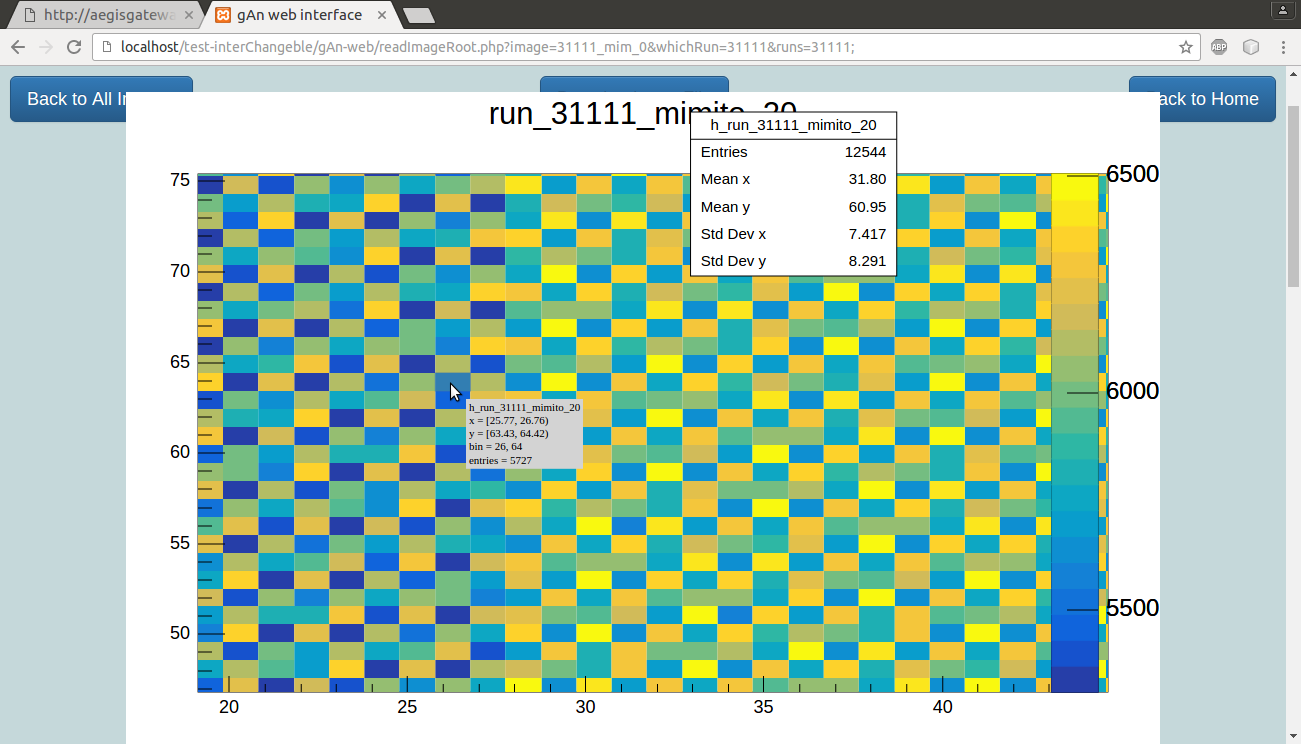
\includegraphics[scale=0.25]{RootLikeImage2.png} 
\caption{Moving the cursor the system shows the value of this histogram in the selected point}
\end{figure}



\begin{figure}[H]
\centering
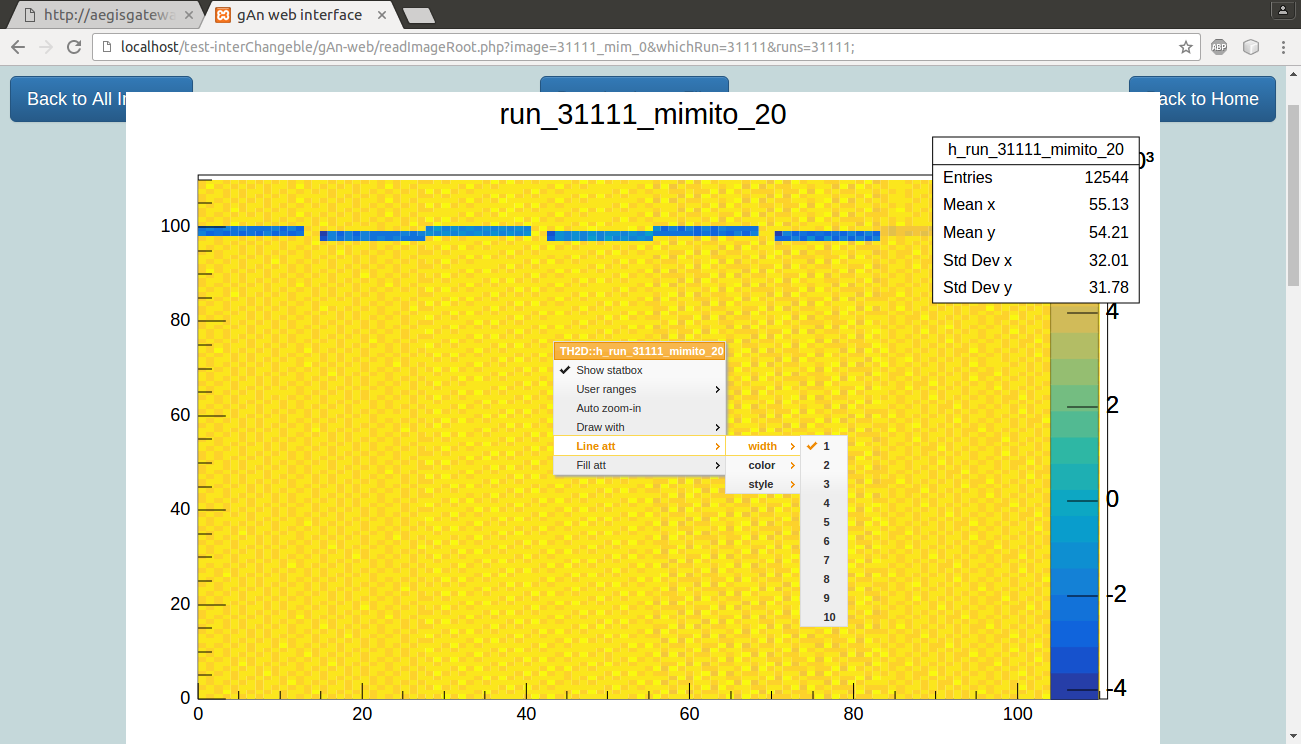
\includegraphics[scale=0.25]{RootLikeImage.png} 
\caption{The user can modify numerous settings in the generated image}
\end{figure}

\begin{figure}[H]
\centering
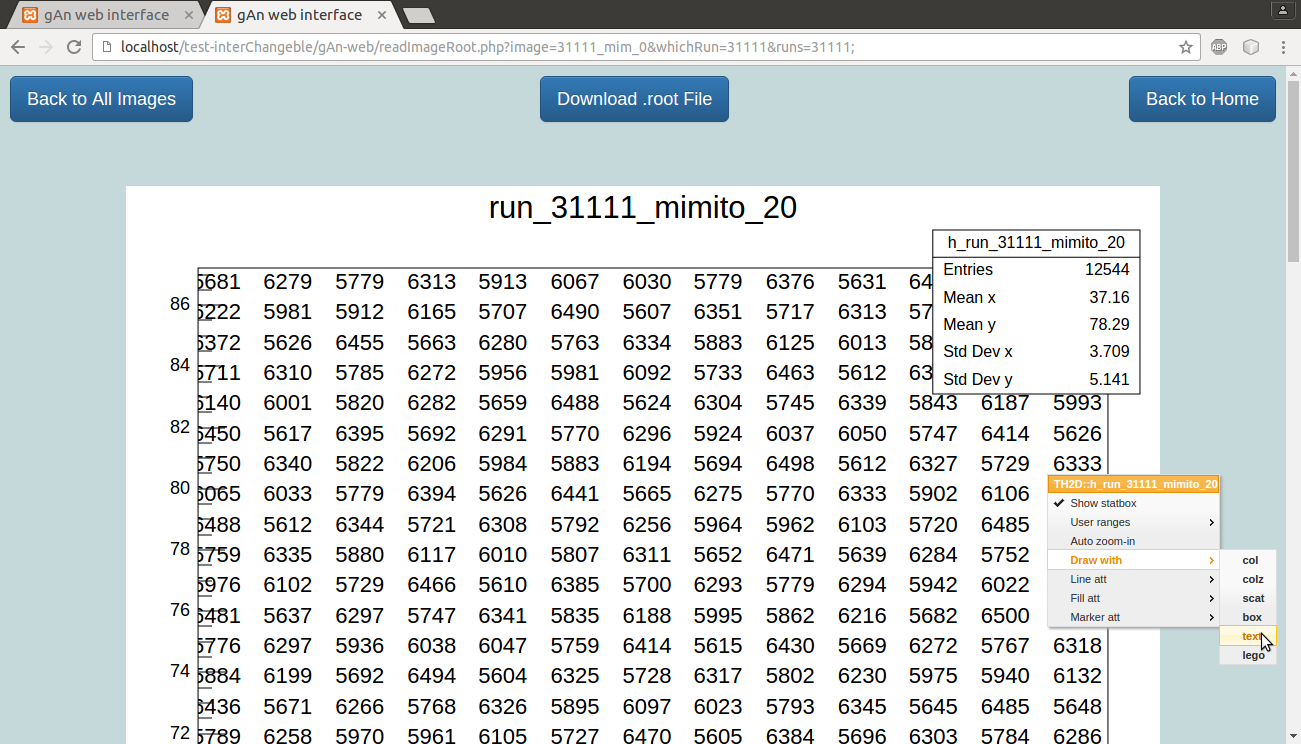
\includegraphics[scale=0.25]{RootLikeImage3.png} %TODO %TODO %TODO %TODO %TODO %TODO take this screen
\caption{The user can show the histogram not only in traditional format, but also in a numerical format where the numbers are the value of the function in their position}
\end{figure}

\begin{figure}[H]
\centering
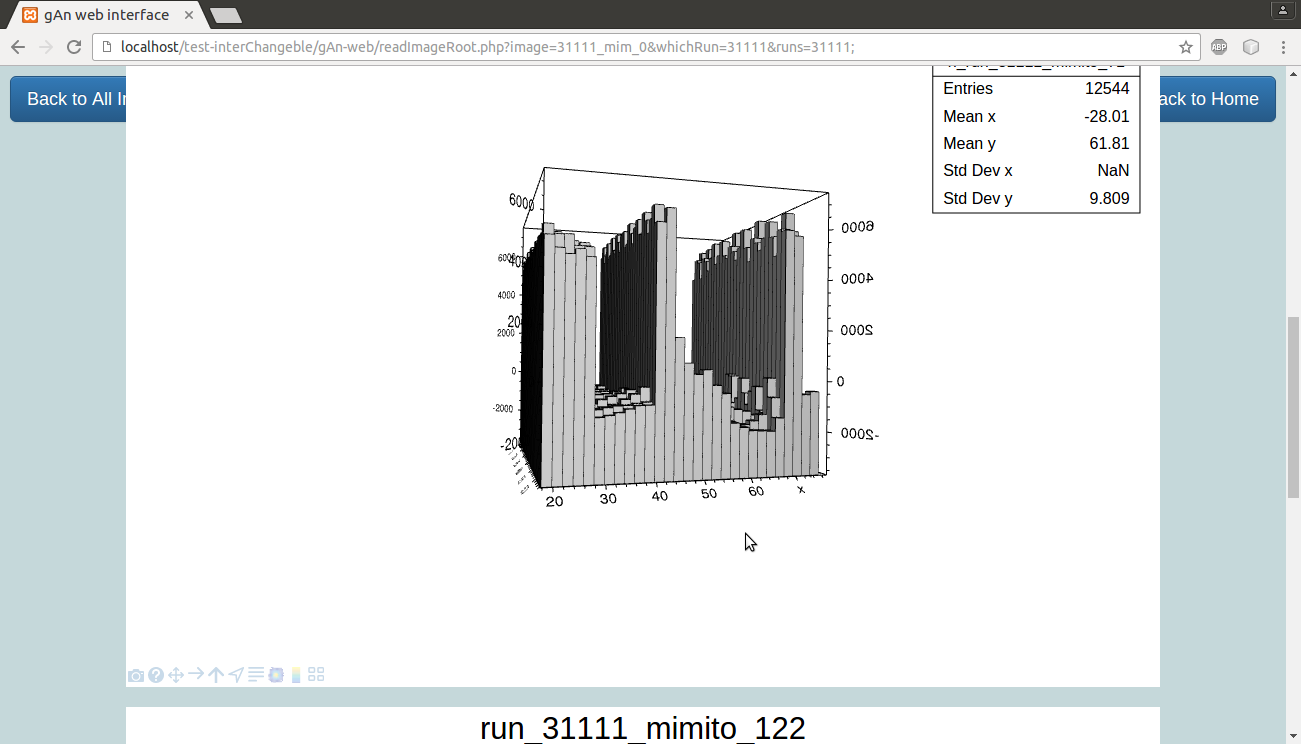
\includegraphics[scale=0.25]{RootLikeImage4.png} %TODO %TODO %TODO %TODO %TODO %TODO %TODO  take this screen
\caption{Another solution is to generate a 3d image in lego-style of the histogram}
\end{figure}


 
\end{enumerate}


\subsection{Added pages}
